\section{Dataset Creation}

In this section, we describe the process for our dataset creation.


\begin{figure*}[t!]
    \centering
    \subfloat[Huam generated \label{fig:realwc}]{
        
\includegraphics[width=.45\textwidth]{wordcloud_Human_story.png}
    }\hspace{1em}
    \subfloat[AI generated\label{fig:realwc} ]{
        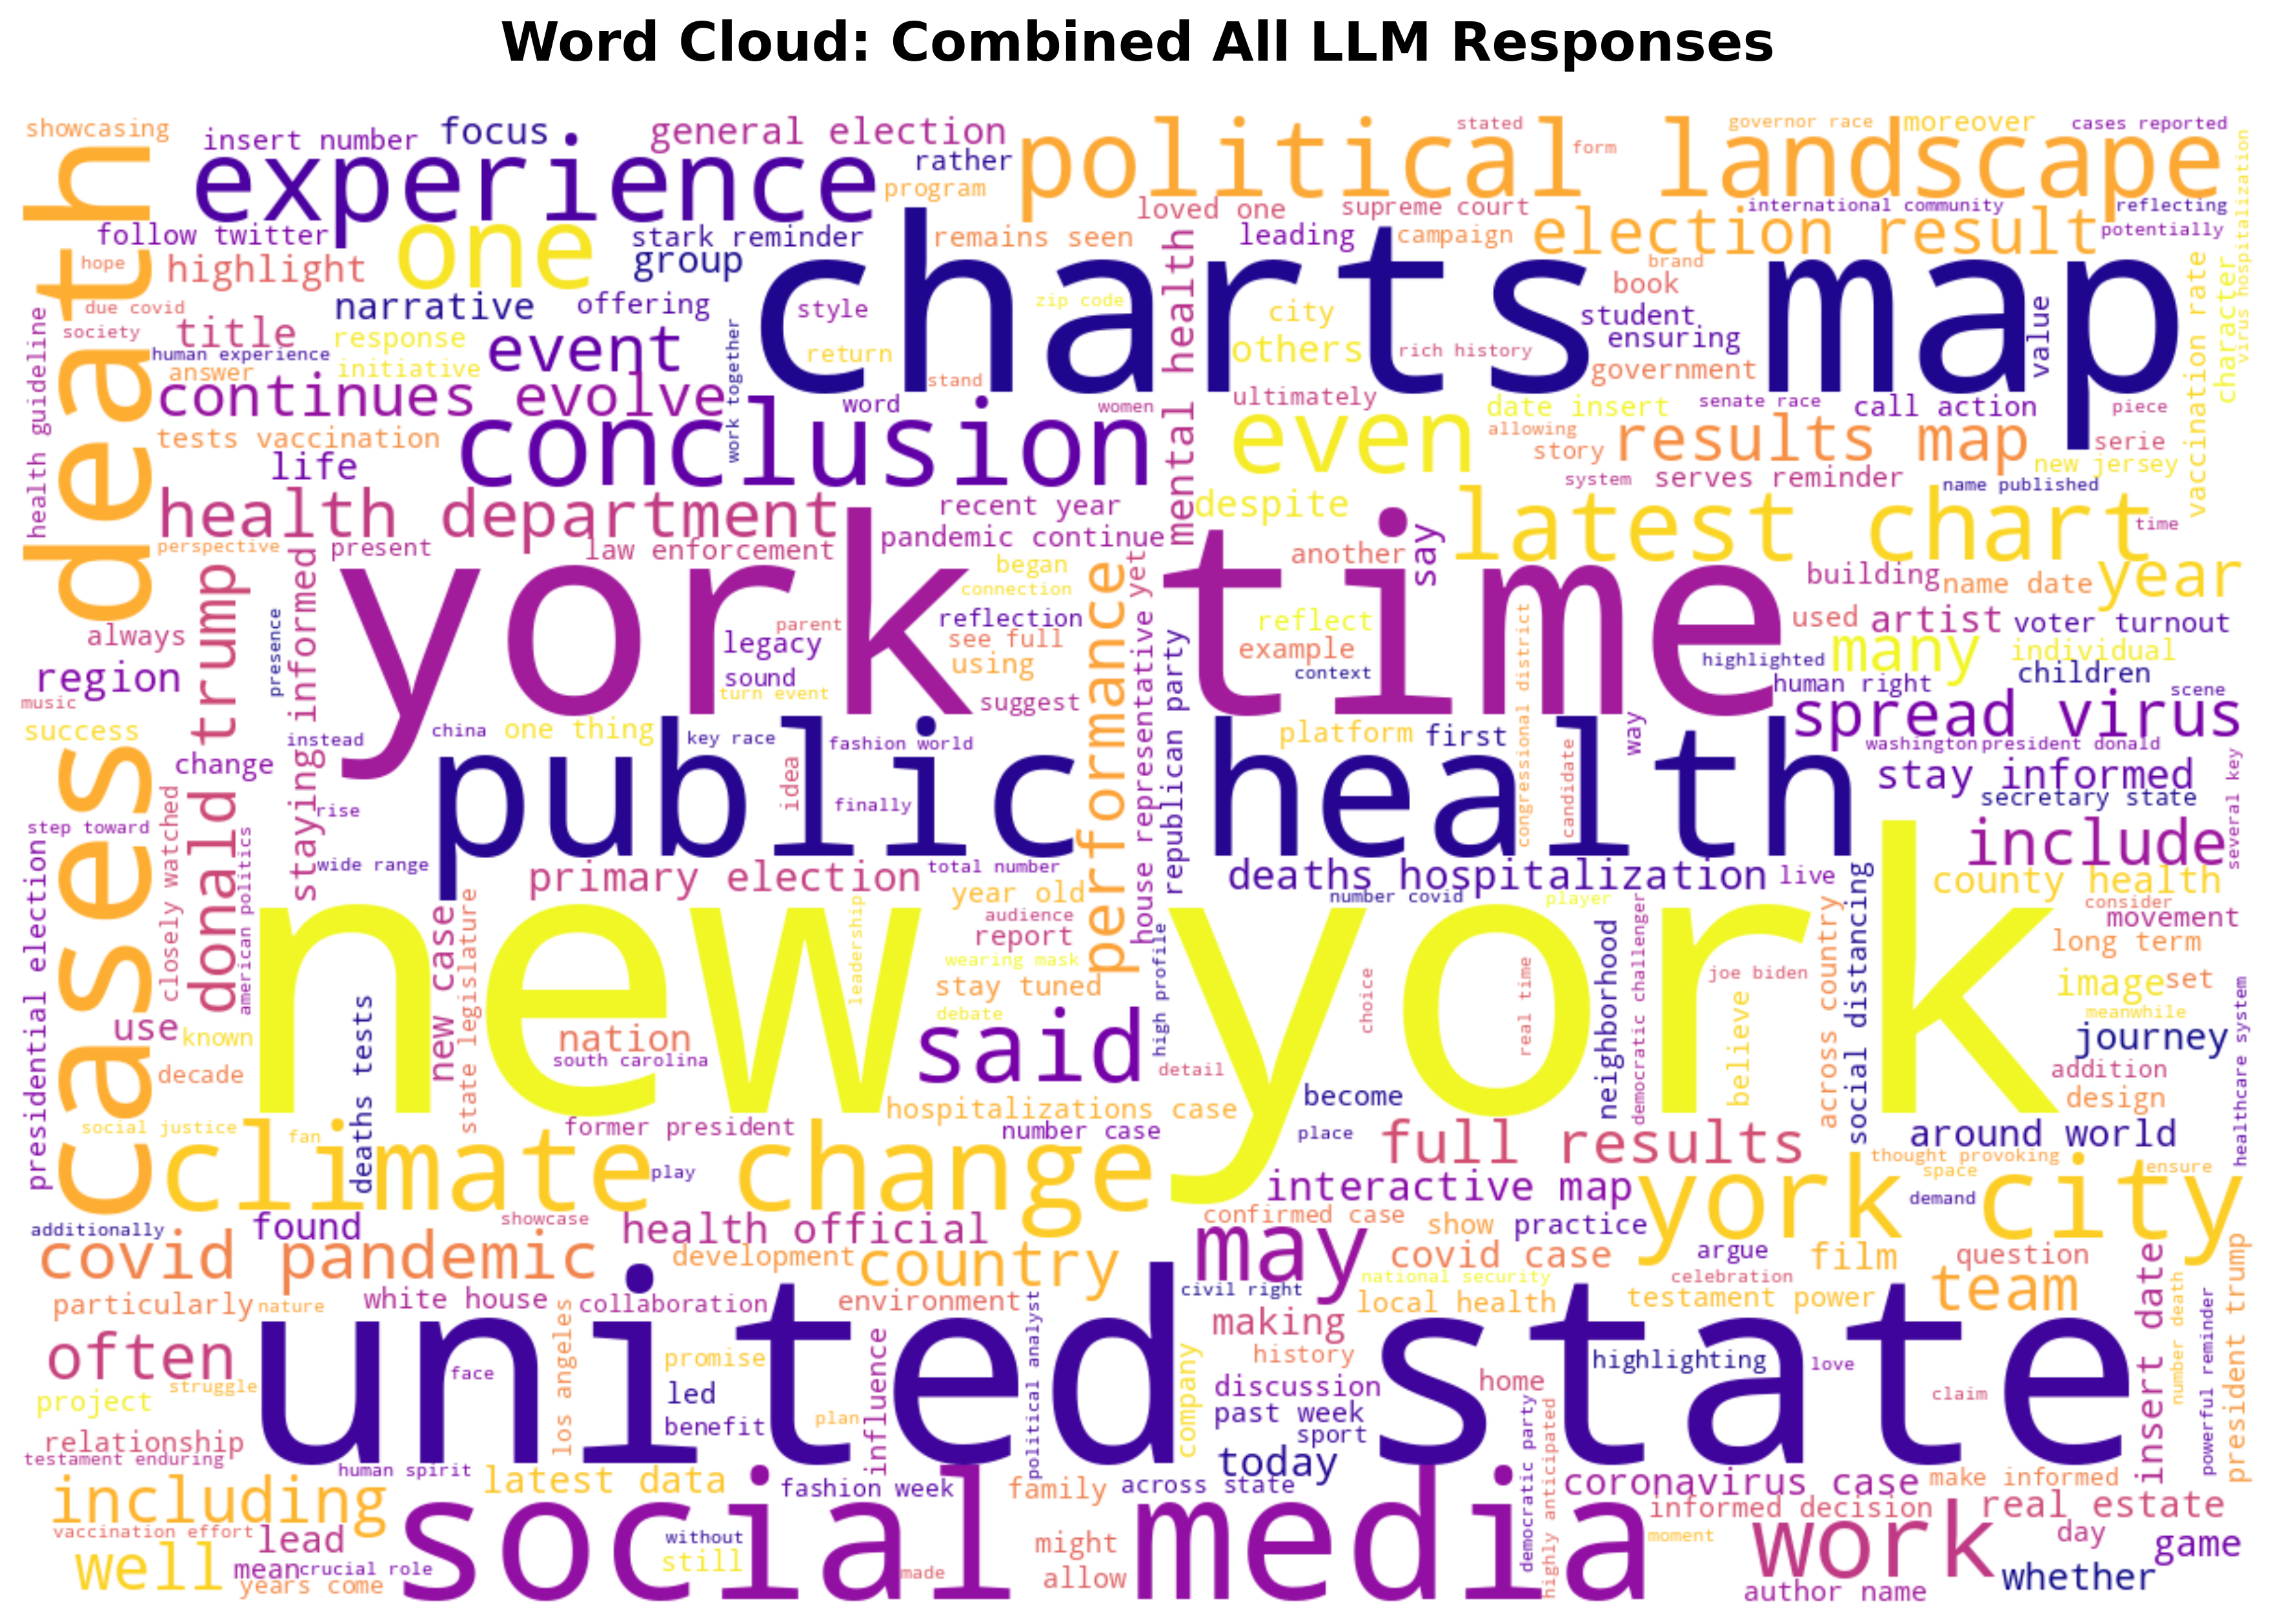
\includegraphics[width=.45\textwidth]{wordcloud_combined_all_llms.png}
    }\hspace{1em}
    \caption{Wordcloud of human written and AI generated text. } 
    \label{fig:wc} 
\end{figure*}

\subsection{base data source}
Our dataset is built upon a large-scale collection of New York Times (NYT) articles spanning January 1, 2000, to the present day. The core NYT dataset comprises over 2.1 million articles and is updated daily, ensuring that the resource remains current and reflective of evolving news trends. Key metadata fields include the abstract of the article, web URL, headline, keywords, publication date, news desk, section name, byline, word count, among other features. These attributes not only capture the diversity of topics covered by the NYT but also provide rich context for further analysis. %Here is the link to our dataset: 



\subsection{Feature Extraction and Transformation}
\paragraph{Abstract as Prompt:} 
The article abstract is extracted and used as a prompt to generate AI text outputs. This serves as a controlled input for language model experiments, ensuring that each generated output is grounded in real-world journalistic content.

\paragraph{Web URL for Human Story Extraction:} 
The provided web URL for each article is utilized to fetch the full human-authored narrative (hereafter referred to as the ``human story''). This extraction captures the in-depth reporting and storytelling inherent to the source material.

\subsection{Generation of AI Texts}
Using the article abstracts as prompts, several state-of-the-art language models were used to generate corresponding texts. The models include Gemma-2-9b, Mistral-7B, Qwen-2-72B, LLaMA-8B, Yi-Large  and GPT\_4-o.

The dataset is thus extended to include both the human-authored text (human story) and AI-generated outputs for direct comparison.

\subsection{Dataset Structure and Statistics}
The final assembled dataset is organized into a tabular format with the following nine columns:
\begin{itemize}
    \item \textbf{Prompt:} The original abstract extracted from the NYT articles.
    \item \textbf{Human\_story:} The full narrative text fetched via the article’s web URL.
    \item \textbf{gemma-2-9b:} AI-generated text produced using the Gemma-2-9b model.
    \item \textbf{mistral-7B:} Output text from the Mistral-7B model.
    \item \textbf{qwen-2-72B:} Text generated by the Qwen-2-72B model.
    \item \textbf{llama-8B:} Output from the LLaMA-8B model.
    \item \textbf{yi-large:} Text generated by the Yi-Large model.
    \item \textbf{gpt\_4-o:} AI-generated output from GPT\_4-o.
\end{itemize}

\begin{table}[h]
\centering
\begin{tabular}{lr}
\hline
\textbf{Column} & \textbf{Count} \\
\hline
Prompt         & 7321 \\
Human\_story   & 7295 \\
Gemma-2-9b     & 7310 \\
Mistral-7B     & 7316 \\
Qwen-2-72B     & 7314 \\
LLaMA-8B       & 7306 \\
Yi-Large       & 7319 \\
GPT\_4-o       & 7321 \\
\hline
\textbf{Total} & 58502 \\
\hline
\end{tabular} 
\caption{Data distribution across real data and varion LLM generated articles. }
\label{tab:aggregated_counts_total}
\end{table}


In total, we have over 58,000 real and synthetic arcitles. The detailed distribution is provided in Table \ref{tab:aggregated_counts_total}. Each LLM contributes roughly equal number of articles.  The dataset is available at:\href{https://huggingface.co/datasets/gsingh1-py/train}{https://huggingface.co/datasets/gsingh1-py/train}.

Figure \ref{fig:wc} shows the wordclouds of human written and AI generated text (combination of all LL generated data) respectively. We can see that key words like "new york", "united state" are prominent across both. 



\subsection{Potential uses of the dataset}
This dataset is uniquely positioned to advance research in the detection of AI-generated content. With a dual composition of human-authored texts (human stories) and AI-generated outputs from multiple state-of-the-art language models, the dataset provides a rich, annotated resource for developing, training, and benchmarking AI content detection systems. Key research directions include:
\begin{itemize}
    \item \textbf{Develop Robust Classifiers:} Create and evaluate models that distinguish between human-written and AI-generated text, improving the transparency and trustworthiness of digital content.
    \item \textbf{Feature Engineering:} Investigate linguistic, stylistic, and semantic features that are indicative of AI generation. This may involve advanced natural language processing techniques and deep learning methods to capture nuanced patterns that differentiate the two text types.
    \item \textbf{Cross-Model Generalization:} Since the dataset includes outputs from multiple language models (e.g., Gemma-2-9b, Mistral-7B, Qwen-2-72B, LLaMA-8B, Yi-Large, GPT\_4-o), it offers a comprehensive basis to study whether detectors trained on one model’s output can generalize to others—a crucial aspect given the rapid evolution of AI text generators.
    \item \textbf{Benchmarking and Model Evaluation:} Benchmark the performance of various AI content detection algorithms by comparing metrics such as precision, recall, and robustness under adversarial conditions.
    \item \textbf{Implications for Misinformation and Authenticity:} In an era where AI-generated text can be misused to spread misinformation or manipulate public opinion, robust detection methods are essential for verifying the authenticity of news content. This dataset supports research that aims to mitigate risks associated with the misuse of AI-generated narratives, reinforcing trust in reputable sources like the New York Times.
    \item \textbf{Hybrid Content Recommendation Systems:} Beyond detection, insights derived from this dataset can inform systems that not only recommend content but also flag or annotate texts based on their origin. This hybrid approach would empower users and platforms to navigate mixed content landscapes more effectively.
\end{itemize}
By combining real-world, human-authored journalism with a spectrum of AI-generated texts, our dataset offers an unprecedented resource for exploring and advancing AI content detection methodologies, ultimately contributing to more secure and transparent information ecosystems.

